
\documentclass{standalone}
\usepackage{amsmath, amsthm, amsfonts, amssymb}
\usepackage{tikz}
\usetikzlibrary{shapes,snakes,positioning,calc}

\newcommand{\disciplina}[6][yellow!20]{
\node [draw=black, fill=#1, very thick, rectangle, rounded corners, inner
sep=03pt, inner ysep=3pt, text width=\the\numexpr #5-6pt, minimum height=40pt,
text centered, anchor=west] (#4) at (#2,#3) {
   \begin{minipage}{\the\numexpr #5-6pt}
   \linespread{1.0}\selectfont
       \centering
       \scriptsize{#6}
   \end{minipage}
};
}

\begin{document}

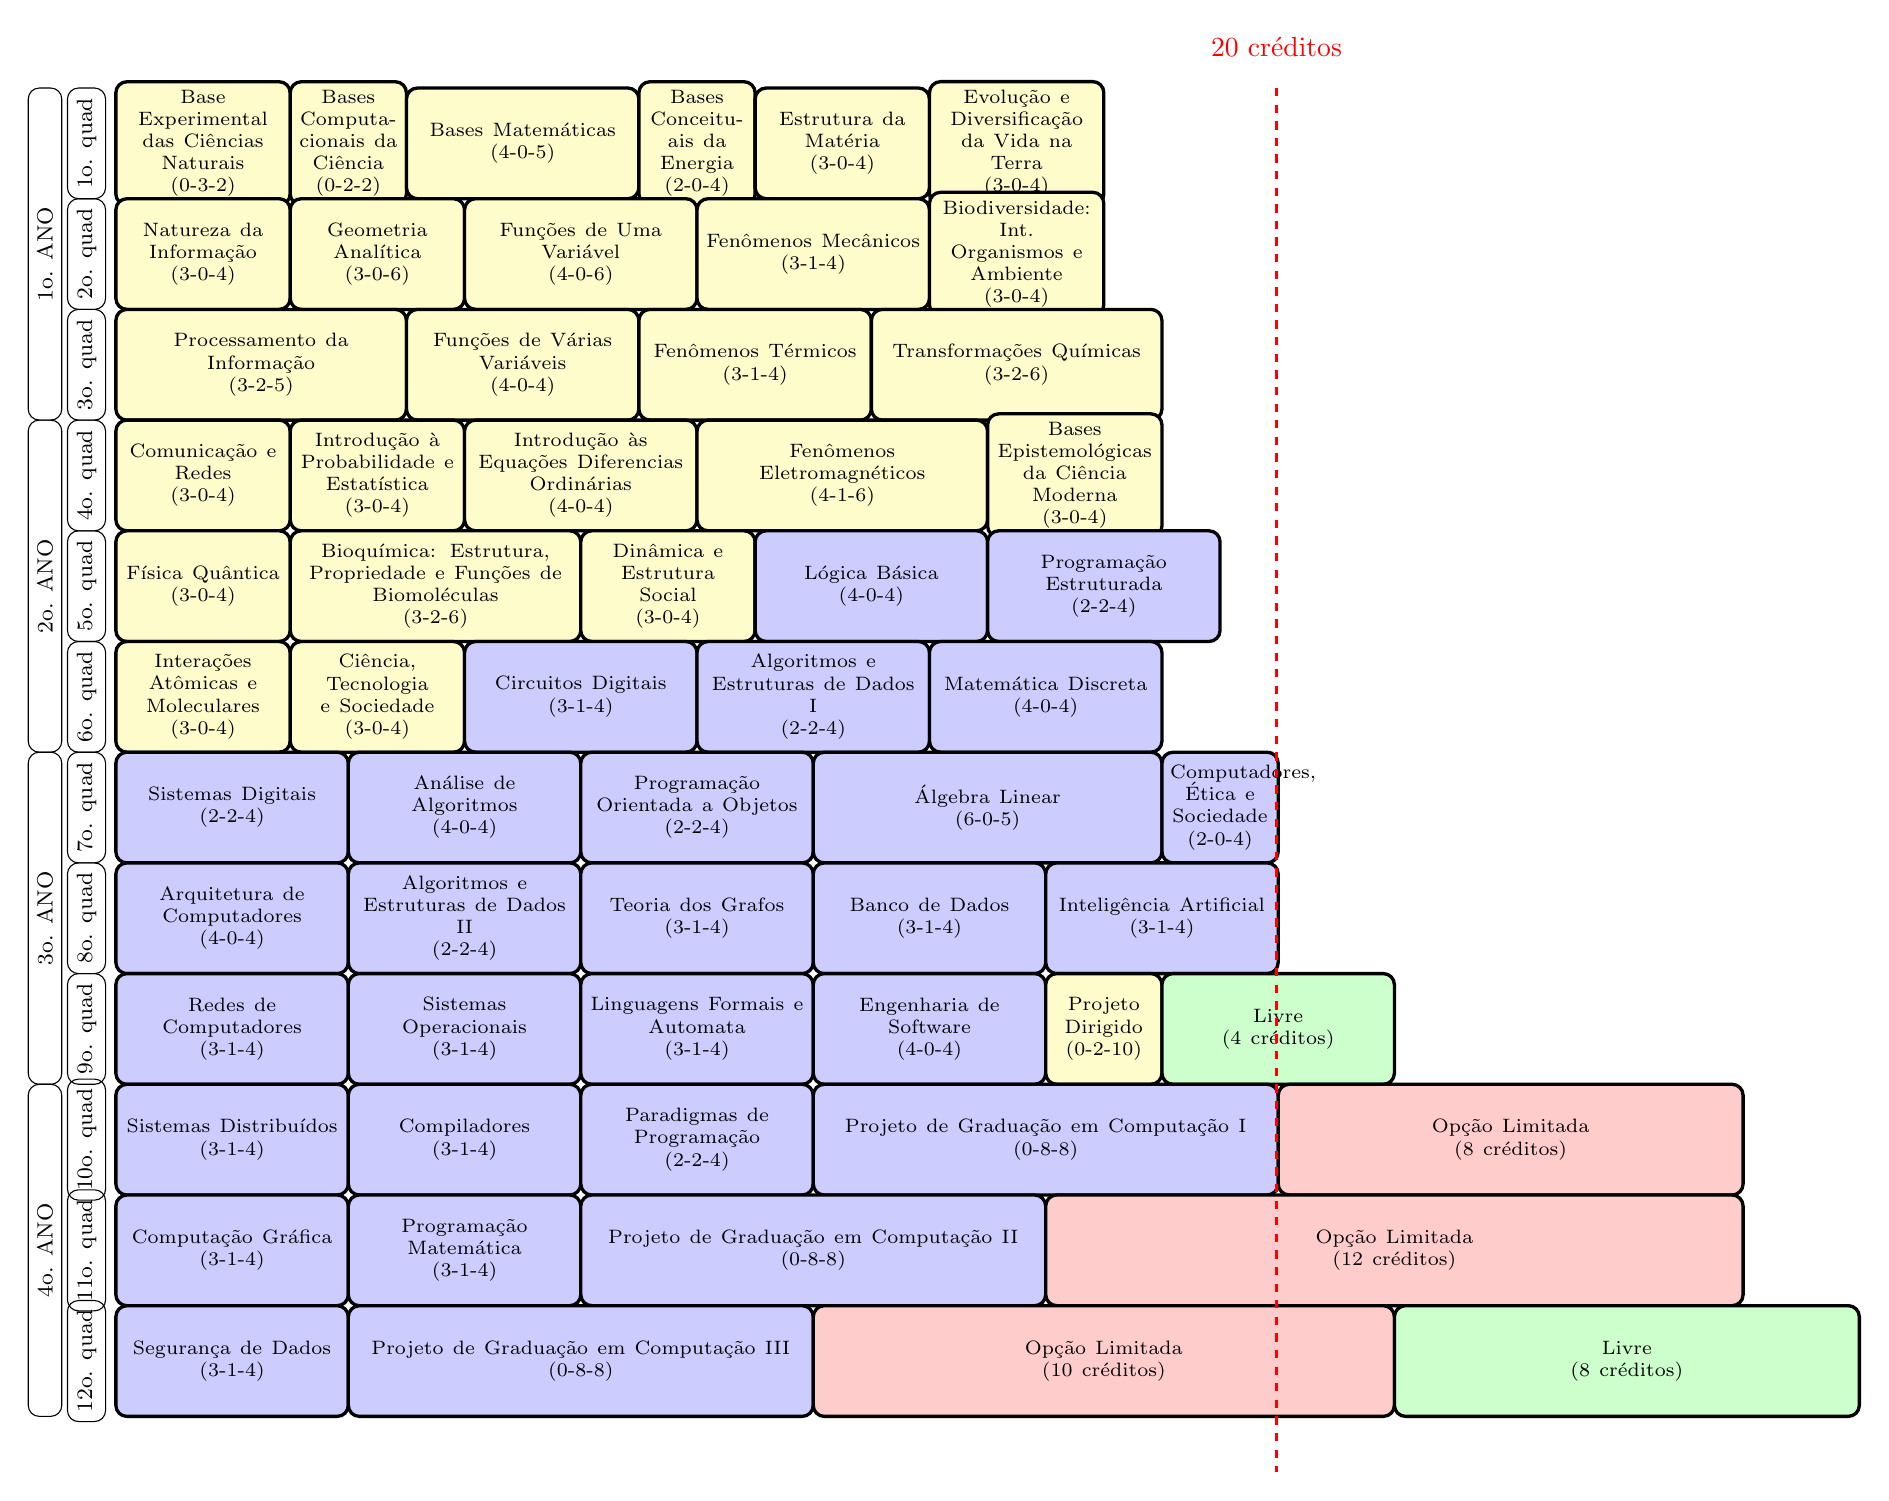
\begin{tikzpicture}
    
    %Q1
    \node [draw, rotate=90, black,rectangle, minimum width=120pt, minimum height=10pt, rounded corners] at (-25pt,-40pt) {\footnotesize{1o. ANO}};
    
    \node [draw, rotate=90, black,rectangle, minimum width=40pt, minimum height=10pt, rounded corners] at (-10pt,0pt) {\footnotesize{1o. quad}};
    
    \disciplina {0pt}{0pt}{a}{63}{Base Experimental das Ciências Naturais\\ (0-3-2)}
    
    \disciplina {63pt}{0pt}{b}{42}{Bases Computacionais da Ciência \\(0-2-2)} 
    
    \disciplina {105pt}{0pt}{c}{84}{Bases Matemáticas\\(4-0-5)}
    
    \disciplina {189pt}{0pt}{d}{42}{Bases Conceituais da Energia \\(2-0-4)}
    
    \disciplina {231pt}{0pt}{e}{63}{Estrutura da Matéria \\(3-0-4)}
    
    \disciplina {294pt}{0pt}{f}{63}{Evolução e Diversificação da Vida na Terra \\(3-0-4)}
    
    
    %Q2
    \node [draw, rotate=90, black,rectangle, minimum width=40pt, minimum height=10pt, rounded corners] at (-10pt,-40pt) {\footnotesize{2o. quad}};
    
    \disciplina [yellow!20]{0pt}{-40pt}{bis0505}{63}{Natureza da Informação\\(3-0-4)}
    
    \disciplina [yellow!20]{63pt}{-40pt}{bis0505}{63}{Geometria Analítica\\(3-0-6)}
    
    \disciplina [yellow!20]{126pt}{-40pt}{bis0505}{84}{Funções de Uma Variável\\(4-0-6)}
    
    \disciplina [yellow!20]{210pt}{-40pt}{bis0505}{84}{Fenômenos Mecânicos\\(3-1-4)}
    
    \disciplina [yellow!20]{294pt}{-40pt}{bis0505}{63}{Biodiversidade: Int. Organismos e Ambiente\\(3-0-4)}
    
    %Q3
    \node [draw, rotate=90, black,rectangle, minimum width=40pt, minimum height=10pt, rounded corners] at (-10pt,-80pt) {\footnotesize{3o. quad}};
    
    \disciplina [yellow!20]{0pt}{-80pt}{bis0505}{105}{Processamento da Informação\\(3-2-5)}
    
    \disciplina [yellow!20]{105pt}{-80pt}{bis0505}{84}{Funções de Várias Variáveis\\(4-0-4)}
    
    \disciplina [yellow!20]{189pt}{-80pt}{bis0505}{84}{Fenômenos Térmicos\\(3-1-4)}
    
    \disciplina [yellow!20]{273pt}{-80pt}{bis0505}{105}{Transformações Químicas\\(3-2-6)}
    
    
    %Q4
    \node [draw, rotate=90, black,rectangle, minimum width=120pt, minimum height=10pt, rounded corners] at (-25pt,-160pt) {\footnotesize{2o. ANO}};
    
    \node [draw, rotate=90, black,rectangle, minimum width=40pt, minimum height=10pt, rounded corners] at (-10pt,-120pt) {\footnotesize{4o. quad}};
    
    \disciplina [yellow!20]{0pt}{-120pt}{bis0505}{63}{Comunicação e Redes\\(3-0-4)}
    
    \disciplina [yellow!20]{63pt}{-120pt}{bis0505}{63}{Introdução à Probabilidade e Estatística\\(3-0-4)}
    
    \disciplina [yellow!20]{126pt}{-120pt}{bis0505}{84}{Introdução às Equações Diferencias Ordinárias\\(4-0-4)}
    
    \disciplina [yellow!20]{210pt}{-120pt}{bis0505}{105}{Fenômenos Eletromagnéticos\\(4-1-6)}
    
    \disciplina [yellow!20]{315pt}{-120pt}{bis0505}{63}{Bases Epistemológicas da Ciência Moderna\\(3-0-4)}
    
    %Q5
    \node [draw, rotate=90, black,rectangle, minimum width=40pt, minimum height=10pt, rounded corners] at (-10pt,-160pt) {\footnotesize{5o. quad}};
    
    \disciplina [yellow!20]{0pt}{-160pt}{bis0505}{63}{Física Quântica\\(3-0-4)}
    
    \disciplina [yellow!20]{63pt}{-160pt}{bis0505}{105}{Bioquímica: Estrutura, Propriedade e Funções de Biomoléculas\\(3-2-6)}
    
    \disciplina [yellow!20]{168pt}{-160pt}{bis0505}{63}{Dinâmica e Estrutura Social\\(3-0-4)}
    
    \disciplina [blue!20]{231pt}{-160pt}{bis0505}{84}{Lógica Básica\\(4-0-4)}
    
    \disciplina [blue!20]{315pt}{-160pt}{bis0505}{84}{Programação Estruturada\\(2-2-4)}
    
    %Q6
    \node [draw, rotate=90, black,rectangle, minimum width=40pt, minimum height=10pt, rounded corners] at (-10pt,-200pt) {\footnotesize{6o. quad}};
    
    \disciplina [yellow!20]{0pt}{-200pt}{bis0505}{63}{Interações Atômicas e Moleculares\\(3-0-4)}
    
    \disciplina [yellow!20]{63pt}{-200pt}{bis0505}{63}{Ciência, Tecnologia \\e Sociedade\\(3-0-4)}
    
    \disciplina [blue!20]{126pt}{-200pt}{bis0505}{84}{Circuitos Digitais\\(3-1-4)}
    
    \disciplina [blue!20]{210pt}{-200pt}{bis0505}{84}{Algoritmos e Estruturas de Dados I\\(2-2-4)}
    
    \disciplina [blue!20]{294pt}{-200pt}{bis0505}{84}{Matemática Discreta\\(4-0-4)}
    
    %Q7
    \node [draw, rotate=90, black,rectangle, minimum width=120pt, minimum height=10pt, rounded corners] at (-25pt,-280pt) {\footnotesize{3o. ANO}};
    
    
    \node [draw, rotate=90, black,rectangle, minimum width=40pt, minimum height=10pt, rounded corners] at (-10pt,-240pt) {\footnotesize{7o. quad}};
    
    \disciplina [blue!20]{0pt}{-240pt}{bis0505}{84}{Sistemas Digitais\\(2-2-4)}
    
    \disciplina [blue!20]{84pt}{-240pt}{bis0505}{84}{Análise de Algoritmos\\(4-0-4)}
    
    \disciplina [blue!20]{168pt}{-240pt}{bis0505}{84}{Programação Orientada a Objetos\\(2-2-4)}
    
    \disciplina [blue!20]{252pt}{-240pt}{bis0505}{126}{Álgebra Linear\\(6-0-5)}
    
    \disciplina [blue!20]{378pt}{-240pt}{bis0505}{42}{Computadores, Ética e Sociedade\\(2-0-4)}
    
    %Q8
    \node [draw, rotate=90, black,rectangle, minimum width=40pt, minimum height=10pt, rounded corners] at (-10pt,-280pt) {\footnotesize{8o. quad}};
    
    \disciplina [blue!20]{0pt}{-280pt}{bis0505}{84}{Arquitetura de Computadores\\(4-0-4)}
    
    \disciplina [blue!20]{84pt}{-280pt}{bis0505}{84}{Algoritmos e Estruturas de Dados II\\(2-2-4)}
    
    \disciplina [blue!20]{168pt}{-280pt}{bis0505}{84}{Teoria dos Grafos\\(3-1-4)}
    
    \disciplina [blue!20]{252pt}{-280pt}{bis0505}{84}{Banco de Dados\\(3-1-4)}
    
    \disciplina [blue!20]{336pt}{-280pt}{bis0505}{84}{Inteligência Artificial\\(3-1-4)}
    
    
    %Q9
    \node [draw, rotate=90, black,rectangle, minimum width=40pt, minimum height=10pt, rounded corners] at (-10pt,-320pt) {\footnotesize{9o. quad}};
    
    
    \disciplina [blue!20]{0pt}{-320pt}{bis0505}{84}{Redes de Computadores\\(3-1-4)}
    
    \disciplina [blue!20]{84pt}{-320pt}{bis0505}{84}{Sistemas Operacionais\\(3-1-4)}
    
    \disciplina [blue!20]{168pt}{-320pt}{bis0505}{84}{Linguagens Formais e Automata\\(3-1-4)}
    
    \disciplina [blue!20]{252pt}{-320pt}{bis0505}{84}{Engenharia de Software\\(4-0-4)}
    
    \disciplina [yellow!20]{336pt}{-320pt}{bis0505}{42}{Projeto Dirigido\\(0-2-10)}
    
    \disciplina [green!20]{378pt}{-320pt}{bis0505}{84}{Livre\\(4 créditos)}
    
    %Q10
    \node [draw, rotate=90, black,rectangle, minimum width=120pt, minimum height=10pt, rounded corners] at (-25pt,-400pt) {\footnotesize{4o. ANO}};
    
    \node [draw, rotate=90, black,rectangle, minimum width=40pt, minimum height=10pt, rounded corners] at (-10pt,-360pt) {\footnotesize{10o. quad}};
    
    
    \disciplina [blue!20]{0pt}{-360pt}{bis0505}{84}{Sistemas Distribuídos\\(3-1-4)}
    
    \disciplina [blue!20]{84pt}{-360pt}{bis0505}{84}{Compiladores\\(3-1-4)}
    
    \disciplina [blue!20]{168pt}{-360pt}{bis0505}{84}{Paradigmas de Programação\\(2-2-4)}
    
    \disciplina [blue!20]{252pt}{-360pt}{bis0505}{168}{Projeto de Graduação em Computação I\\(0-8-8)}
    
    \disciplina [red!20]{420pt}{-360pt}{bis0505}{168}{Opção Limitada\\(8 créditos)}
    
    %Q11
    \node [draw, rotate=90, black,rectangle, minimum width=40pt, minimum height=10pt, rounded corners] at (-10pt,-400pt) {\footnotesize{11o. quad}};
    
    
    \disciplina [blue!20]{0pt}{-400pt}{bis0505}{84}{Computação Gráfica\\(3-1-4)}
    
    \disciplina [blue!20]{84pt}{-400pt}{bis0505}{84}{Programação Matemática\\(3-1-4)}
    
    \disciplina [blue!20]{168pt}{-400pt}{bis0505}{168}{Projeto de Graduação em Computação II\\(0-8-8)}
    
    \disciplina [red!20]{336pt}{-400pt}{bis0505}{252}{Opção Limitada\\(12 créditos)}
    
    %Q12
    \node [draw, rotate=90, black,rectangle, minimum width=40pt, minimum height=10pt, rounded corners] at (-10pt,-440pt) {\footnotesize{12o. quad}};
    
    \disciplina [blue!20]{0pt}{-440pt}{bis0505}{84}{Segurança de Dados\\(3-1-4)}
    
    \disciplina [blue!20]{84pt}{-440pt}{bis0505}{168}{Projeto de Graduação em Computação III\\(0-8-8)}
    
    \disciplina [red!20]{252pt}{-440pt}{bis0505}{210}{Opção Limitada\\(10 créditos)}
    
    \disciplina [green!20]{462pt}{-440pt}{bis0505}{168}{Livre\\(8 créditos)}
    
    \draw [red,thick,dashed] (420pt,20pt) -- (420pt,-480pt); 
    \node [text=red] at (420pt,35pt) {20 créditos};
    
    
\end{tikzpicture}

\end{document}
